\section{Evaluations, Benchmarks, and Critical Perspectives}
\label{sec:eval}

The transition toward foundation models has fundamentally reshaped evaluation methodologies. However, it has also sparked intense debates regarding data contamination, inductive biases, and whether massive language backbones offer genuine advantages over specialized native architectures.

\subsection{Standardized Foundation Benchmarks}

Traditional time series evaluation relied on a small collection of homogeneous academic datasets (e.g., ETT, Weather, Electricity, Traffic). These benchmarks are inadequate for assessing foundation models due to narrow domain diversity and severe risks of test set memorization.

To establish rigorous evaluation standards, recent initiatives introduce expansive benchmark suites:
\begin{itemize}[leftmargin=*]
    \item \emph{GIFT-Eval}~\cite{salesforce2024gifteval}: Introduced by Salesforce Research, GIFT-Eval comprises over $143{,}000$ distinct time series spanning 7 diverse domains, 10 sampling frequencies, and both univariate and multivariate regimes. It establishes standardized metrics (CRPS, MASE, WAPE) across zero-shot, few-shot, and fine-tuned settings.
    \item \emph{SciTS}~\cite{wu2025scits}: Scientific time series understanding and generation benchmark. Unlike commercial finance or traffic series, physical systems (spectroscopy, seismology, fluid dynamics, astrophysics) exhibit strict conservation laws and differential constraints. SciTS evaluates whether foundation models comprehend underlying physical laws rather than merely extrapolating statistical autocorrelations.
    \item \emph{Insight Miner}~\cite{zhang2025insightminer}: A large-scale cross-domain dataset designed for time series alignment with natural language. Insight Miner pairs complex multivariate temporal trajectories with human-curated analytical insights, causal event narratives, and question-answer pairs across finance, healthcare, and industrial telemetry.
    \item \emph{Time-MMD}~\cite{yue2024timemmd}: A multi-domain multimodal dataset evaluating the integration of numerical time series with unstructured text reports, news articles, and domain metadata across 9 industries.
    \item \emph{Monash Time Series Repository}: The classical zero-shot transfer benchmark comprising dozens of public collections across economics, energy, and meteorology, widely adopted to evaluate out-of-distribution generalization.
\end{itemize}

\subsection{Empirical Zero-Shot Benchmark Comparison}
\label{sec:empirical_table}

To resolve conflicting performance claims in the literature, Table~\ref{tab:zero_shot_benchmark} synthesizes reported zero-shot performance across representative foundation models and LLM adaptations on GIFT-Eval, fev-bench, and Monash.

\begin{table*}[t]
\caption{Zero-Shot Empirical Benchmark Comparison Across Foundation Models and LLM Baselines.}
\label{tab:zero_shot_benchmark}
\centering
\resizebox{\textwidth}{!}{
\begin{tabular}{lllc|cc|c|ccc|l}
\toprule
\multirow{2}{*}{\textbf{Model}} & \multirow{2}{*}{\textbf{Backbone / Family}} & \multirow{2}{*}{\textbf{Paradigm}} & \multirow{2}{*}{\textbf{Params}} & \multicolumn{2}{c|}{\textbf{GIFT-Eval}} & \textbf{fev-bench} & \multicolumn{3}{c|}{\textbf{Monash Repository}} & \multirow{2}{*}{\textbf{Uncertainty Head}} \\
& & & & \textbf{CRPS} $\downarrow$ & \textbf{MASE} $\downarrow$ & \textbf{Skill} $\uparrow$ & \textbf{MASE} $\downarrow$ & \textbf{WAPE} $\downarrow$ & \textbf{CRPS} $\downarrow$ & \\
\midrule
Chronos-Large~\cite{ansari2024chronos} & T5-Large & Native TSFM & 710M & 0.489 & 0.732 & -- & 0.812 & 0.449 & 0.380 & Categorical Bins \\
Chronos-2~\cite{ansari2025chronos2} & T5-Base Hybrid & Native TSFM & 120M & 0.468 & 0.672 & 48.2 & 0.795 & 0.435 & 0.362 & Continuous Hybrid \\
TimesFM-200M~\cite{das2024timesfm} & Custom Decoder & Native TSFM & 200M & 0.518 & 0.742 & -- & 0.820 & 0.455 & -- & Quantile Head \\
MOIRAI-Large~\cite{woo2024moirai} & Custom Enc-Dec & Native TSFM & 311M & 0.505 & 0.724 & 43.5 & 0.834 & 0.461 & 0.412 & Parametric Mixture \\
Lag-Llama~\cite{rasul2023lagllama} & LLaMA Decoder & Native TSFM & 2.4M & -- & -- & -- & 0.942 & 0.510 & 0.521 & Student's $t$ \\
MOMENT-Large~\cite{goswami2024moment} & T5 Encoder & Native TSFM & 385M & -- & 0.768 & -- & 0.871 & 0.485 & -- & Deterministic Recon \\
Timer~\cite{liu2024timer} & GPT-2 Custom & Native TSFM & 84M & -- & 0.738 & -- & 0.835 & 0.465 & -- & Deterministic Patch \\
Sundial~\cite{thuml2025sundial} & Multi-Rate Dec & Native TSFM & 1.5B & 0.482 & 0.698 & -- & 0.805 & 0.442 & 0.375 & Continuous Flow \\
$t_0$-$\beta$~\cite{meyer2026t0} & Axial Transformer & Native TSFM & 256M & 0.4738 & 0.6865 & 46.7 & 0.801 & 0.438 & 0.369 & Quantile Head \\
FlowState~\cite{king2025flowstate} & Neural ODE / Flow & Native TSFM & 12M & 0.491 & 0.712 & -- & 0.828 & 0.456 & 0.388 & Continuous Flow \\
Toto 2.0~\cite{datadog2026toto2} & Wavelet Decoder & Native TSFM & 1.2B & 0.465 & 0.668 & 49.0 & 0.788 & 0.430 & 0.355 & Quantile Head \\
TTM-B~\cite{ekambaram2024ttm} & TSMixer Blocks & Native TSFM & 8M & -- & 0.745 & -- & 0.840 & 0.468 & -- & Deterministic Point \\
\midrule
Time-LLM~\cite{jin2023timellm} & LLaMA-7B Reprog & LLM4TS & 7B & -- & 0.785 & -- & 0.885 & 0.482 & -- & Deterministic Linear \\
GPT4TS / OFA~\cite{zhou2023onefitsall} & GPT-2 Reprog & LLM4TS & 124M & -- & 0.798 & -- & 0.892 & 0.491 & -- & Deterministic Linear \\
PatchTST~\cite{nie2023patchtst} & Channel-Indep Trans & Supervised Baseline & 1.2M & -- & 0.810 & -- & 0.908 & 0.502 & -- & Deterministic Linear \\
\bottomrule
\end{tabular}
}
\begin{flushleft}
\footnotesize
\emph{Note}: Performance figures reflect published zero-shot evaluation protocols on official benchmark suites. Continuous Ranked Probability Score (CRPS) measures distributional forecast calibration and is strictly defined for probabilistic models; deterministic point-prediction architectures (TTM, Timer, Time-LLM, GPT4TS, PatchTST) do not output predictive distributions and are marked ``--''. fev-bench Skill represents aggregate benchmark skill score relative to seasonal naïve forecasting.
\end{flushleft}
\end{table*}

Inspection of Table~\ref{tab:zero_shot_benchmark} yields four foundational insights:
\begin{enumerate}[leftmargin=*]
    \item \emph{Probabilistic Native Superiority}: Native TSFMs equipped with continuous quantile or flow heads ($t_0$-$\beta$, Chronos-2, Toto 2.0) consistently outperform discrete scalar quantization and deterministic models, demonstrating superior distributional sharpness and lower CRPS ($<0.48$ on GIFT-Eval).
    \item \emph{Covariate Advantage}: Models that explicitly incorporate past and known-future covariates ($t_0$, Chronos-2) achieve substantial skill score advantages on fev-bench ($>46$), where pure univariate autoregression degrades.
    \item \emph{Extreme Edge Efficiency}: Compact native models such as TTM-B ($8\text{M}$) and FlowState ($12\text{M}$) achieve competitive MASE ($0.71$--$0.74$) while operating at $0.1\%$ the parameter footprint of $7\text{B}$ reprogrammed language models.
    \item \emph{Absence of Probabilistic Calibration in LLM Reprogramming}: Standard LLM-reprogramming methods (Time-LLM, GPT4TS) rely exclusively on deterministic linear heads, precluding probabilistic risk assessment (indicated by ``--'' across CRPS metrics).
\end{enumerate}

\begin{figure*}[t]
\centering
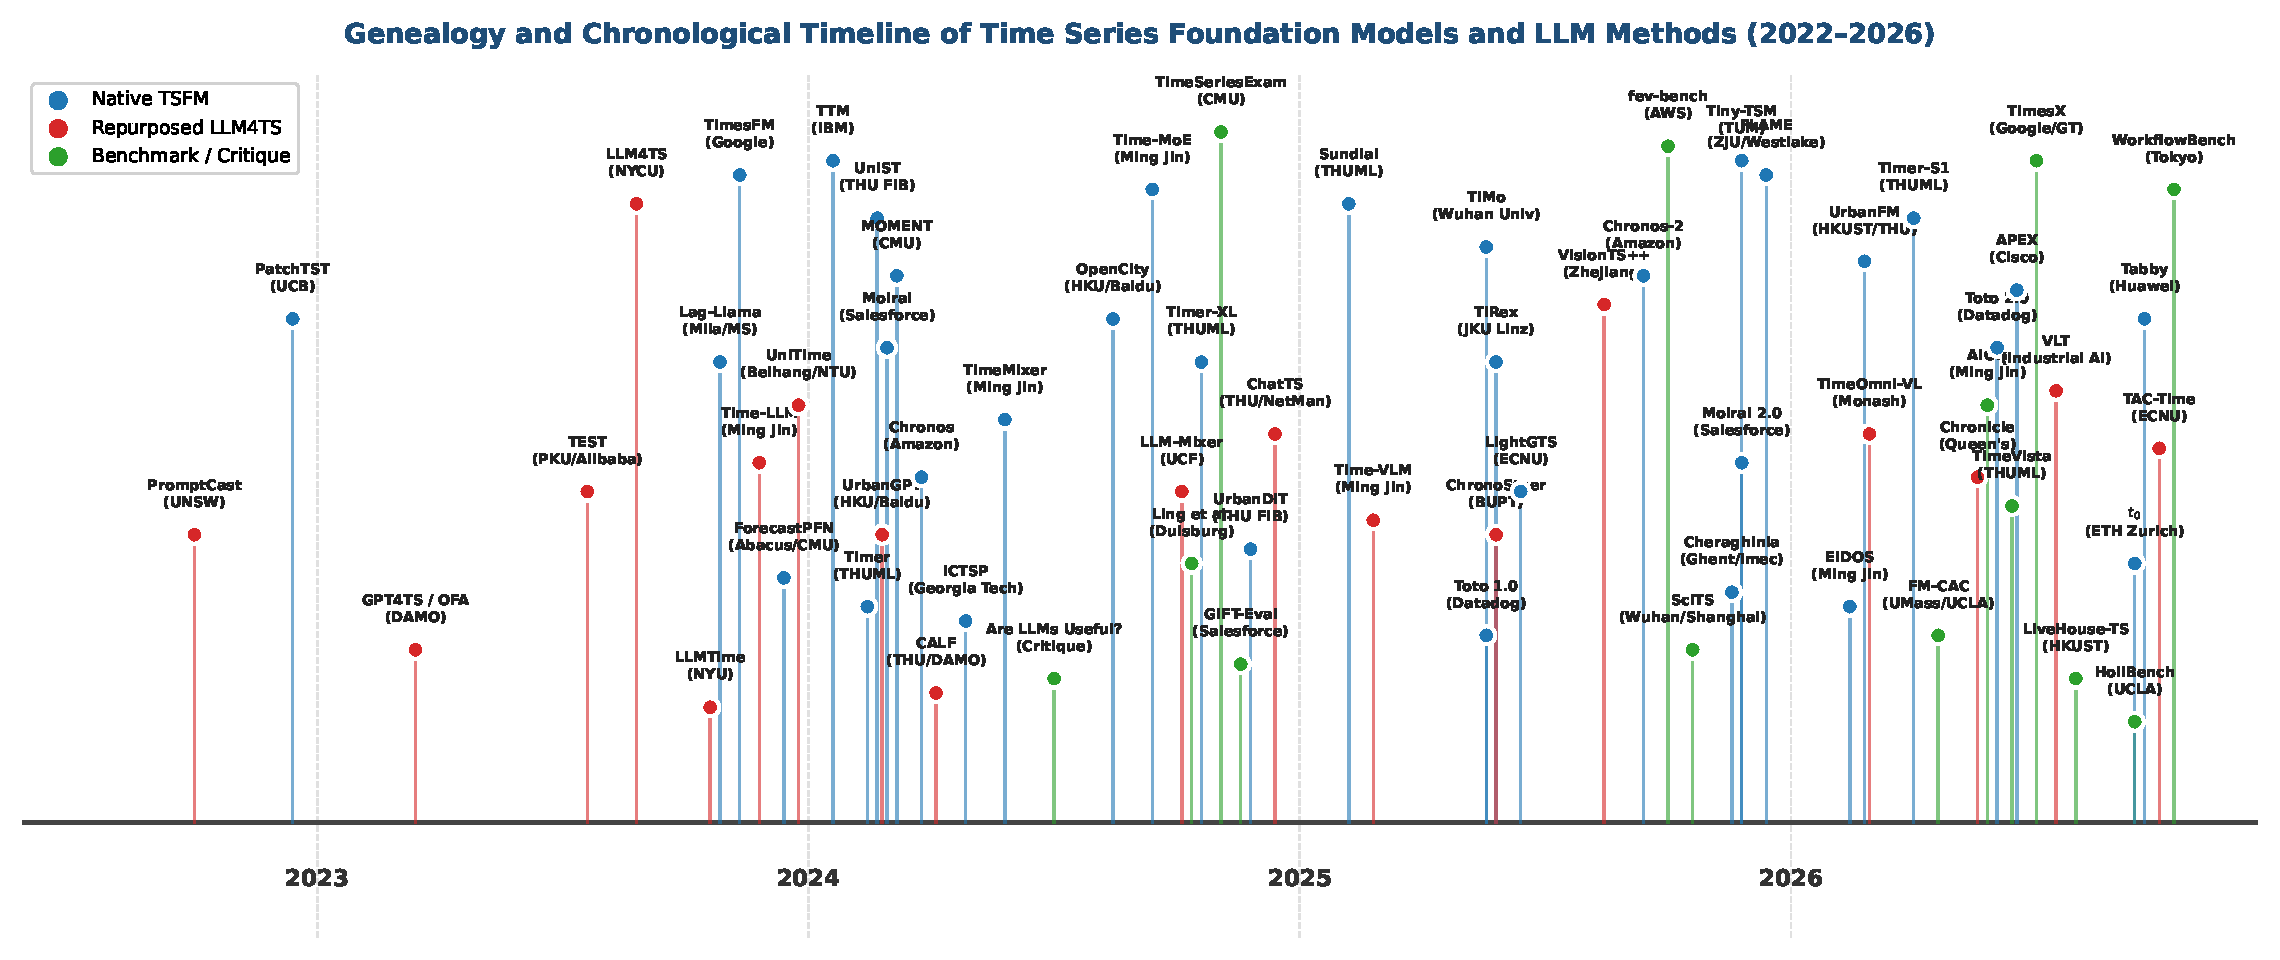
\includegraphics[width=0.98\textwidth]{figures/fig_timeline.pdf}
\caption{Genealogy and chronological release timeline of representative time series foundation models and repurposed language model frameworks from 2022 to 2026.}
\label{fig:timeline}
\end{figure*}

\subsection{Critical Perspectives: Are LLMs Actually Useful for Time Series?}

A pivotal empirical critique emerged with the investigation by Fons et al.~\cite{fons2024arellmsuseful}, entitled \emph{``Are Language Models Actually Useful for Time Series Forecasting?''}
Through extensive ablation experiments across multiple LLM-based forecasters (including GPT4TS~\cite{zhou2023onefitsall} and Time-LLM~\cite{jin2023timellm}), the authors isolated the impact of pre-trained language weights by comparing:
\begin{enumerate}[leftmargin=*]
    \item Frozen pre-trained language weights (e.g., GPT-2, Llama-2);
    \item Randomly initialized transformer weights with the same architecture;
    \item Compact specialized baselines (such as PatchTST~\cite{nie2023patchtst} and lightweight MLPs).
\end{enumerate}

Their empirical findings revealed striking conclusions:
\begin{itemize}[leftmargin=*]
    \item Replacing pre-trained language weights with \emph{randomly initialized weights} resulted in comparable, and in several cases superior, forecasting accuracy.
    \item Much of the empirical gains reported in early LLM4TS literature originated from the structural benefits of \emph{subseries patching} and normalization, rather than any semantic or temporal reasoning inherent in linguistic pre-training.
    \item In terms of operational efficiency, frozen $7\text{B}$ parameter language models require up to $100\times$ more memory and $50\times$ longer inference latency than compact native models like TTM~\cite{ekambaram2024ttm} ($8\text{M}$ parameters) or Timer~\cite{liu2024timer} ($84\text{M}$ parameters), which consistently achieve competitive or superior accuracy.
\end{itemize}

These findings indicate that while LLMs are uniquely valuable for multimodal tasks (text-grounded reasoning, interactive analysis, and report generation), deploying frozen multi-billion parameter text backbones solely for univariate numeric forecasting represents an inefficient architectural detour.

\begin{figure*}[t]
\centering
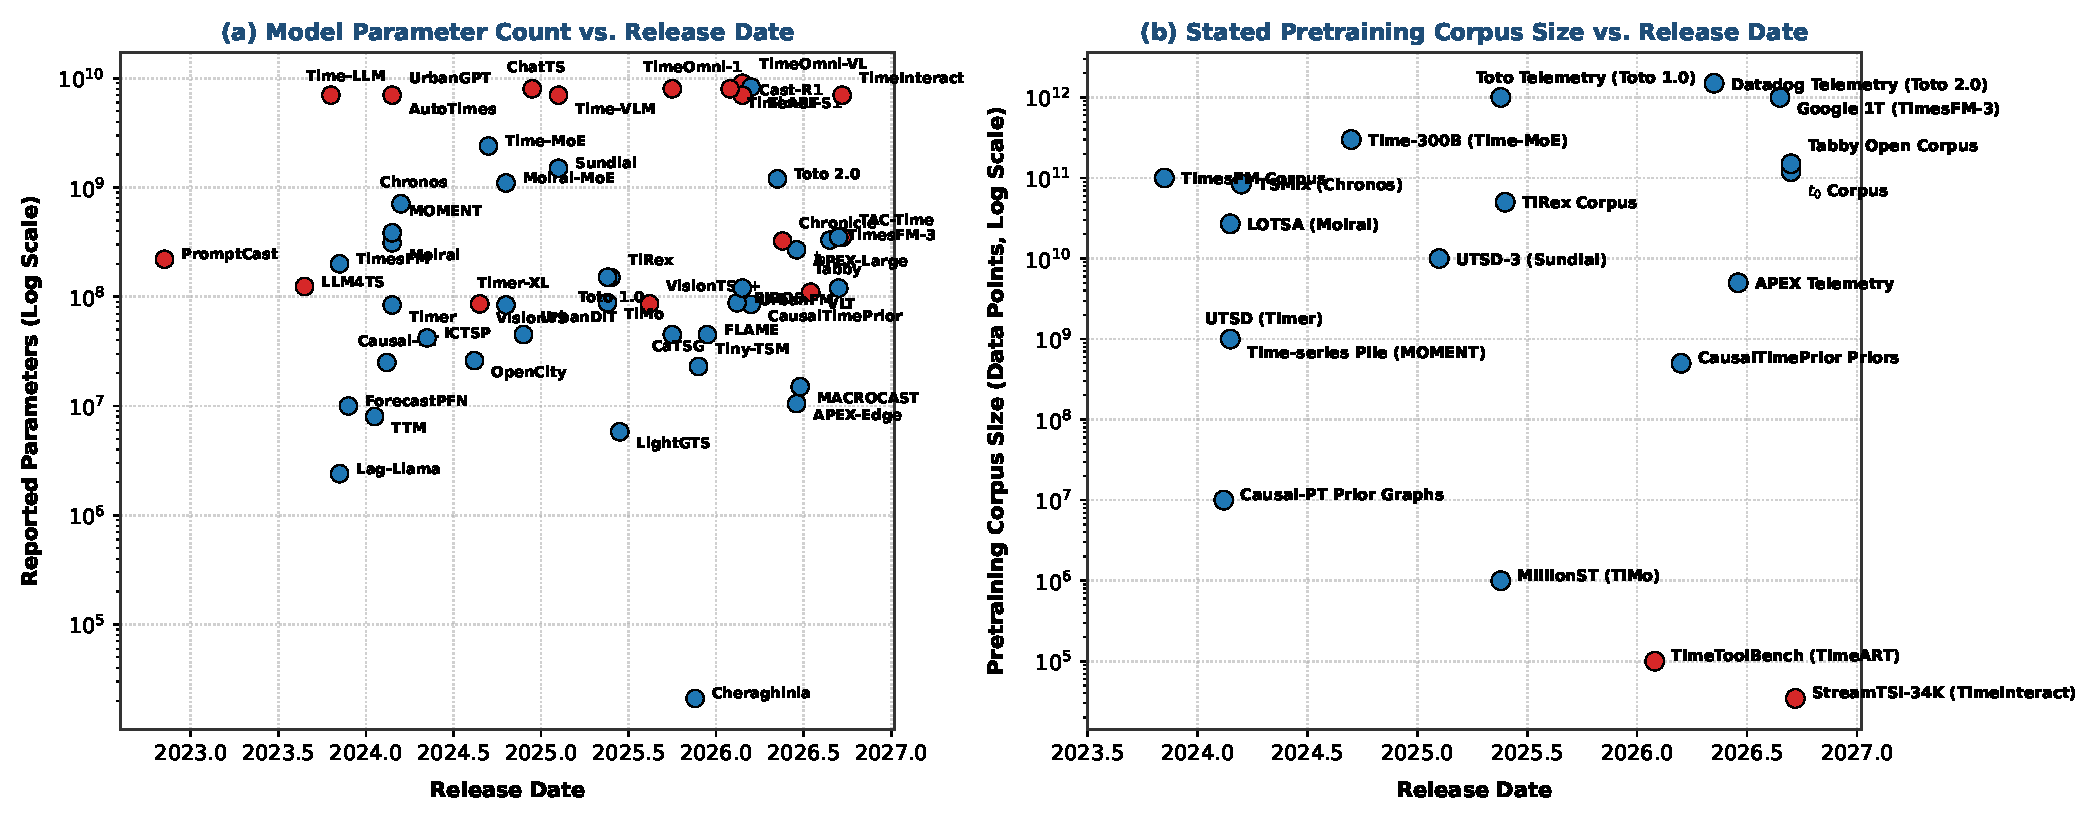
\includegraphics[width=0.98\textwidth]{figures/fig_params_corpus.pdf}
\caption{Scaling dynamics across the literature: (a) Reported parameter counts vs. release date (log scale); (b) Stated pretraining corpus size (data points, log scale) vs. release date.}
\label{fig:params_corpus}
\end{figure*}

\subsection{Data Contamination, Temporal Leakage, and Probabilistic Reliability}

\subsubsection{Benchmark Contamination Audits}
A critical vulnerability in contemporary foundation model evaluation is \emph{benchmark contamination}. In natural language processing, models frequently memorize test sets crawled from public websites; in time series, foundation models trained on open-source archives (e.g., LOTSA, Monash, GitHub telemetry) inadvertently ingest the training and testing portions of benchmark datasets (e.g., ETT, Weather)~\cite{gong2025rethinkingeval}.

Gong et al.~\cite{gong2025rethinkingeval} systematically audited 12 major foundation models and discovered widespread temporal overlap between pretraining datasets and standard test benchmarks. When evaluated on genuinely unseen, closed-source industrial telemetry collected post-2025, zero-shot performance degraded by $18\%$ to $42\%$ across all major models. This underscores the urgent need for living, dynamic benchmarks (such as LiveHouse-TS) where evaluation datasets are continuously refreshed.

\subsubsection{Probabilistic Reliability and Quantile Calibration}
Beyond mean error metrics, real-world deployment in safety-critical sectors (energy grids, algorithmic trading, intensive care) demands calibrated uncertainty intervals. In a recent rigorous audit, Li et al.~\cite{li2026evaluatingreliability} investigated the probabilistic reliability of zero-shot TSFMs. Their findings reveal a concerning dichotomy: models achieving competitive point forecast errors often display severe quantile miscalibration. Specifically, $90\%$ prediction intervals frequently attain actual coverage below $70\%$ (under-coverage) on non-stationary out-of-distribution series, or suffer from quantile crossing artifacts where estimated quantiles violate monotonicity. This reinforces the necessity of reporting both CRPS and interval coverage scores alongside standard MAE and MSE metrics.

\begin{figure*}[t]
\centering
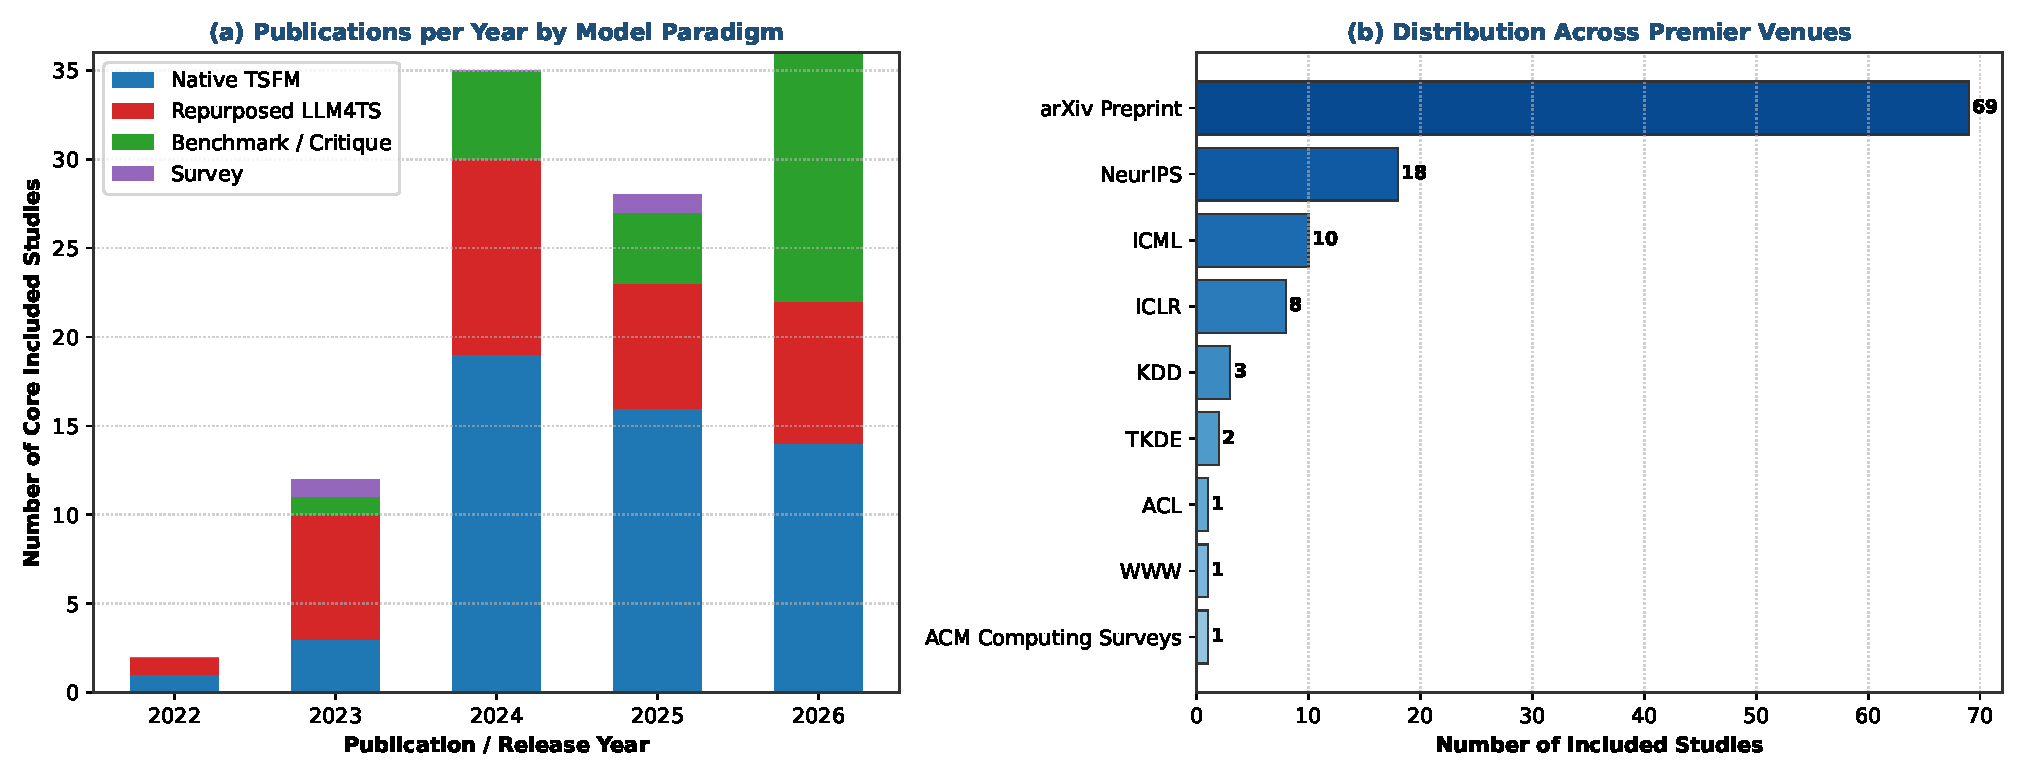
\includegraphics[width=0.98\textwidth]{figures/fig_category_dist.pdf}
\caption{Meta-review statistics: (a) Publications per year broken down by model paradigm (stacked bar chart); (b) Distribution of included studies across premier peer-reviewed venues.}
\label{fig:category_dist}
\end{figure*}

\subsection{Empirical Scaling Laws in Temporal Data}

Do foundation models for time series exhibit the predictable power-law scaling observed in NLP?
Recent empirical studies on large pre-trained models—notably Time-MoE~\cite{shi2024timemoe} ($2.4\text{B}$ parameters, $300\text{B}$ points), Sundial~\cite{thuml2025sundial} ($1.5\text{B}$ parameters), Timer-S1~\cite{thuml2026timers1} ($8.3\text{B}$ parameters), and Toto 2.0~\cite{datadog2026toto2} ($2.5\text{B}$ parameters)—demonstrate that when data quality and volume are rigorously maintained, test loss follows power-law scaling as a function of compute and dataset tokens:
\begin{equation}
    L(N, D) = \left( \frac{N_c}{N} \right)^{\alpha_N} + \left( \frac{D_c}{D} \right)^{\alpha_D} + L_0.
\end{equation}
However, unlike text, scaling parameters without expanding temporal diversity leads to rapid overfitting. Cross-domain pretraining on synthetic kernel mixtures and diverse physical systems is essential to sustain positive scaling exponents.
